%%% StratifiedCV.tex --- 
%% Version: $Id: Stratified.tex,v 0.0 2011/12/21 11:45:27 tangboyun Exp$
%% Copyright : (c) 2011 Boyun Tang
%% License : BSD-style
\documentclass{standalone}
\usepackage{tikz}
\usetikzlibrary{mindmap,shadows,shapes.arrows,shapes.geometric,shapes.misc,matrix,arrows,positioning,calc,decorations.pathreplacing}
\usepackage{graphicx}
\usepackage{xcolor}
\usepackage{times}
\usepackage{verbatim}
\begin{document}
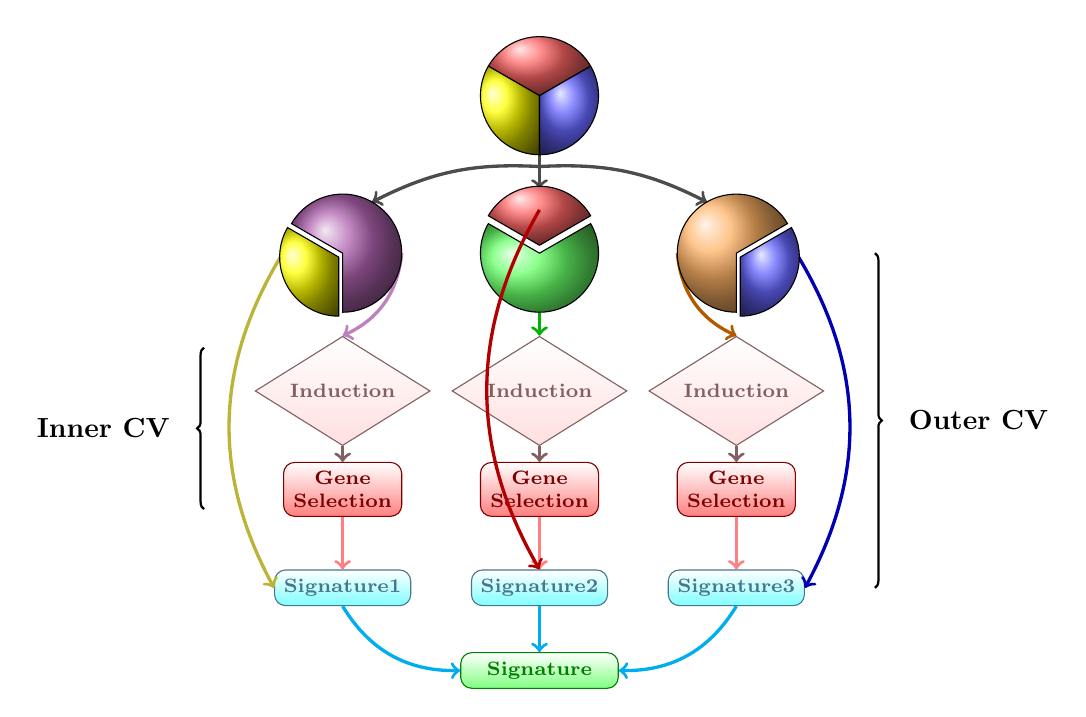
\begin{tikzpicture}[
  se/.style={circular sector,minimum size=1.5cm,circular sector angle=120,shape border uses incircle},
  r/.style={ball color=red!60},
  g/.style={ball color=green!60},
  b/.style={ball color=blue!60},
  or/.style={ball color=orange!60},
  vio/.style={ball color=violet!60},
  ye/.style={ball color=yellow},
  cl/.style={diamond,font=\scriptsize,aspect=1.6,top color=white, bottom color=pink!50,
    draw=pink!50!black!100,text=pink!50!black!100,},
  po/.style={rectangle,font=\scriptsize,rounded corners,top color=white, bottom color=red!50,
    draw=red!50!black!100,text=red!50!black!100,
    minimum width=1.5cm},
  ev/.style={rectangle,font=\scriptsize,rounded corners,top color=white, bottom color=cyan!50,
    draw=cyan!50!black!100,text=cyan!50!black!100,
    minimum width=1.5cm},
  av/.style={ellipse,font=\scriptsize,minimum width=2cm,rectangle,rounded corners,top color=white, bottom color=green!50,
    draw=green!50!black!100,text=green!50!black!100,},
  ]

  \node at (-2.5,-3.75) [cl] (cl1) {\textbf{Induction}};
  \node at (0,-3.75) [cl] (cl2) {\textbf{Induction}};  
  \node at (2.5,-3.75) [cl] (cl3) {\textbf{Induction}};  
  
  \node at (-2.5,-5) [po,align=center] (po1) {\textbf{Gene}\\
    \textbf{Selection}};
  \node at (0,-5) [po,align=center] (po2) {\textbf{Gene}\\
    \textbf{Selection}};
  \node at (2.5,-5) [po,align=center] (po3) {\textbf{Gene}\\
    \textbf{Selection}};
  
  \node at (-2.5,-6.25) [ev] (ev1) {\textbf{Signature1}};
  \node at (0,-6.25) [ev] (ev2) {\textbf{Signature2}};  
  \node at (2.5,-6.25) [ev] (ev3) {\textbf{Signature3}};  
  \draw  (cl1.south) edge [->,pink!50!black,very thick] (po1.north);
  \draw  (cl2.south) edge [->,pink!50!black,very thick] (po2.north);
  \draw  (cl3.south) edge [->,pink!50!black,very thick] (po3.north);
  \draw  (po1.south) edge [->,red!50,very thick] (ev1.north);
  \draw  (po2.south) edge [->,red!50,very thick] (ev2.north);
  \draw  (po3.south) edge [->,red!50,very thick] (ev3.north);
  
  \node at (0,-7.3) [av] (av1){\textbf{Signature}};
  \draw  (ev1.south) edge [->,cyan,very thick,bend right] (av1.west);
  \draw  (ev2.south) edge [->,cyan,very thick] (av1.north);
  \draw  (ev3.south) edge [->,cyan,very thick,bend left] (av1.east);
  \draw  (0,-0.75) edge [->,black!70,very thick,] (0,-1.18);
  \draw  (0,-0.9) edge [->,black!70,very thick,bend right=15] (-2.125,-1.35);
  \draw  (0,-0.9) edge [->,black!70,very thick,bend left=15] (2.125,-1.35);
  
  \draw  (0,-2.75) edge [->,green!70!black,very thick,] (cl2.north);
  \draw  (-3.26,-2) edge [->,yellow!70!black,very thick,bend right] (ev1.west);
  \draw  (3.26,-2) edge [->,blue!70!black,very thick,bend left] (ev3.east);
  \draw  (1.75,-2) edge [->,orange!70!black,very thick,bend right] (cl3.north);
  \draw  (-1.75,-2) edge [->,red!50!blue!50,very thick,bend left] (cl1.north);
  \draw[r] (0,0) -- (30:.75cm) arc (30:150:.75cm) -- (0,0);
  \draw[ye] (0,0) -- (150:.75cm) arc (150:270:.75cm) -- (0,0);
  \draw[b] (0,0) -- (30:.75cm) arc (30:-90:.75cm) -- (0,0);
  \draw[vio,xshift=-2.5cm,yshift=-2cm] (0,0) -- (-90:.75cm) arc (-90:150:.75cm) -- (0,0);
  \draw[ye,xshift=-2.55cm,yshift=-2.05cm] (0,0) -- (150:.75cm) arc (150:270:.75cm) -- (0,0);
  \draw[r,yshift=-1.9cm] (0,0) -- (30:.75cm) arc (30:150:.75cm) -- (0,0);
  \draw[g,yshift=-2cm] (0,0) -- (-210:.75cm) arc (-210:30:.75cm) -- (0,0);
  \draw[or,xshift=2.5cm,yshift=-2cm] (0,0) -- (30:.75cm) arc (30:270:.75cm) -- (0,0);
  \draw[b,xshift=2.55cm,yshift=-2.05cm] (0,0) -- (30:.75cm) arc (30:-90:.75cm) -- (0,0);
  \draw  (0,-1.45) edge [->,red!70!black,very thick,bend right] (ev2.north);        
  \draw[decorate,decoration={brace},thick] (4.26,-2) to
  node[midway,right,xshift=0.3cm] (bracket) {\textbf{Outer CV}}
  (4.26,-6.25);

  \draw[decorate,decoration={brace},thick] (-4.26,-5.25) to
  node[midway,left,xshift=-0.3cm] (bracket) {\textbf{Inner CV}}
  (-4.26,-3.2);
  
\end{tikzpicture}
\end{document}
